\chapter{System Overview}
In this chapter we give an overview to our system. The system is splitted independent parts, the frontend and backend. The frontend is the whole webinterface for the user designed with HTML, Javascript and CSS. The backend consists out of the commucation interface between frontend and backend for which we used REST API and the database server by itself.

\begin{figure}[hb]
	\centering
		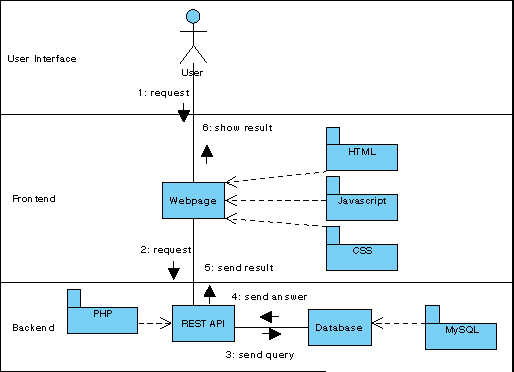
\includegraphics[scale=1.5]{content/graphics/system_overview.pdf}
	\caption{An overview of how requests are handled.}
    \label{fig:system_overview}
\end{figure}

A normal procedure in our system would be that an user of our system uses a functionality of the webinterface to send an command to our REST API. The REST API will now check the valitity of the command and if it is confirmed it will forward an request to the MySQL server. The MySQL server sends the result of the request back the REST API where an answer gets wrapped with the important information and sends it back to the user.
